\usepackage{xcolor}
\usepackage{afterpage}
\usepackage{pifont,mdframed}
\usepackage[bottom]{footmisc}

\makeatletter
\gdef\this@inputfilename{input}
\gdef\this@outputfilename{output}
\makeatother

\lstset{
  basicstyle=\ttfamily,
  columns=fullflexible
}

\setcounter{@subtaskcounter}{-1}

%%%%%%%%%%%%%%%%%%%%%%%%%%%%%%%%%%%%%%%%%%%%%%%%%%%%%%%%%%%%%%%
%%%%%%%%%%%%%%%%%%%%%%%%%%%%%%%%%%%%%%%%%%%%%%%%%%%%%%%%%%%%%%%

Egy állatkertben $N$ rozmár \footnote{románul ,,\textit{morse}''} ül szépen egy sorban. A rozmárokat $0$-tól $N-1$-ig számozzuk.
%In an unspecified zoo, there are $N$ walruses\footnote{"\textit{morse}" in Romanian} sitting neatly in a line. The walruses are numbered from $0$ to $N-1$.

\begin{figure}[H]
    \centering
    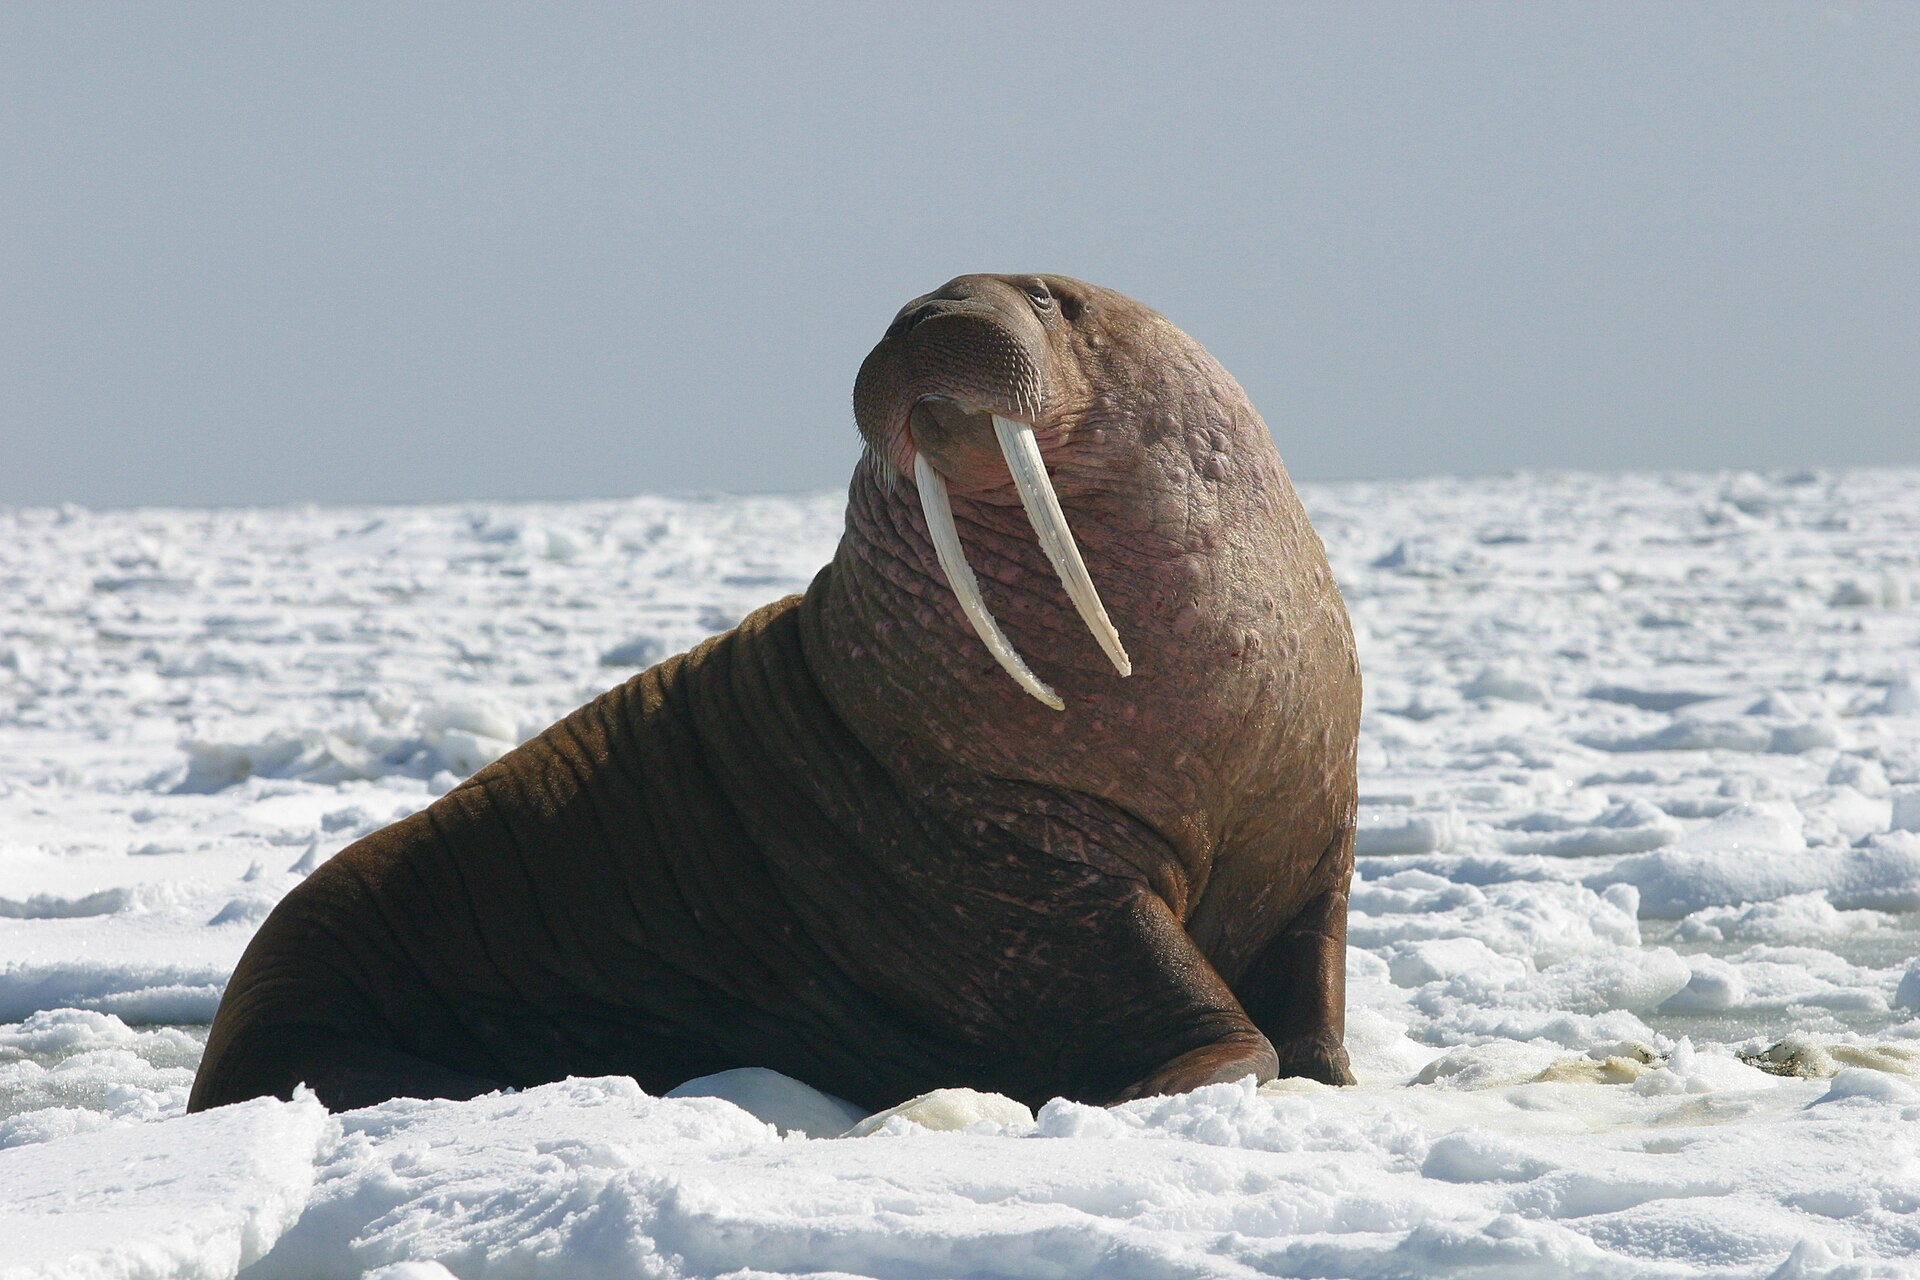
\includegraphics[width=0.6\linewidth]{walrus.jpg}
    \caption{\emph{Odobenus Rosmarus}, más néven \emph{rozmár}.}
\end{figure}

A rozmárok állapotát egy $N$ karakterből álló $\overline{c_0c_1\ldots c_{N-1}}$ karakterlánc jellemzi, ahol:
%The state of the walruses are denoted by a string of $N$ characters $\overline{c_0c_1\ldots c_{N-1}}$, where:
\begin{itemize}
\item $c_i=$\texttt{'.'}, ha az $i$.~rozmár alszik,
%$c_i=$\texttt{'.'}, if walrus $i$ is sleeping; or
\item $c_i=$\texttt{'-'}, ha az $i$.~rozmár ébren van.
%$c_i=$\texttt{'-'}, if walrus $i$ is awake.
\end{itemize}

Minden másodpercben a következő két dolog történik:
%In each second, the following two things happen:
\begin{enumerate}
\item választhatsz egy alvó rozmárt, és felébresztheted,
%you can choose to wake up a walrus yourself; and
\item minden olyan rozmár, amelyiket az előző másodpercben felébresztett valaki, felébreszti a szomszédait. (Azok a rozmárok, amelyek a legelején ébren voltak, \textbf{sohasem} ébresztik fel a szomszédaikat.)
%every walrus that was awakened \textbf{in the previous second} wakes up its neighbours. The walruses which were awake at the start will \textbf{never} wake up their neighbours.
\end{enumerate}

Minden rozmárt szeretnénk ébren látni. Mivel a rozmárok felébresztése veszélyes, a következő kérdésekre szeretnénk választ kapni:
%Since waking up the walruses yourself is dangerous, you ask yourself the following questions:
\begin{enumerate}
\item Legkevesebb hány rozmárt kell felébresztened ahhoz, hogy garantáltan végül minden rozmár felébredjen?
%What is the smallest number of walruses you need to wake up yourself to guarantee that every walrus will be awake eventually?
\item Ha a lehető legkevesebb rozmárt ébreszted fel, mi a legkorábbi lehetséges időpont (másodpercekben), amikor minden rozmár felébred?
%When waking up as few walruses yourself as possible, what is the earliest possible time (in seconds) when all of the walruses will be awake?
\end{enumerate}

\begin{warning}
Az értékelő rendszerből letölthető csatolmányok közt találhatsz
\texttt{morse.*} nevű fájlokat, melyek a bemeneti adatok beolvasását valósítják meg az egyes programnyelveken.
A megoldásodat ezekből a hiányos minta implementációkból kiindulva is elkészítheted.
\end{warning}
%\begin{warning}
%Among the attachments of this task you may find a template file \texttt{morse.*} with a sample incomplete implementation.
%\end{warning}

\InputFile

Minden teszt több tesztesetet tartalmaz. A bemenet első sora egyetlen egész számot tartalmaz a tesztesetek $T$ számát.
%Each test contains multiple test cases. The first line of input contains a single integer $T$, the number of test cases.

Minden teszteset első sora egyetlen egész számot tartalmaz, a rozmárok $N$ számát.

Minden teszteset második sora egy $N$ karakterből álló $\overline{c_0c_1\ldots c_{N-1}}$ karakterláncot tartalmaz.

%The first line of each test case contains a single integer $N$, the number of walruses.
%The second line of each test case contains a string of $N$ characters $\overline{c_0c_1\ldots c_{N-1}}$.

\OutputFile

Minden tesztesethez írj ki két szóközzel elválasztott egész számot egy sorba:
\begin{enumerate}
\item a legkisebb számot, amennyi rozmár felébresztése elég ahhoz, hogy végül mindegyik felébredjen
\item a legkorábbi lehetséges időpont (másodpercben), amikor az összes rozmár felébred ebben az esetben.
\end{enumerate}
%For each test case, print two space separated integers in a line:
%\begin{enumerate}
%\item the minimum number of walruses you need to wake up yourself; and
%\item the earliest possible time (in seconds) when all of the walruses will be awake in this case.
%\end{enumerate}

\Scoring
A megoldásodat sok különböző tesztesetre lefuttatjuk. A tesztesetek részfeladatokba vannak csoportosítva. Egy-egy részfeladatot akkor tekintünk megoldottnak, ha volt legalább egy olyan beadásod, amely az adott részfeladat minden tesztesetére helyes megoldást adott.
A feladat összpontszámát a megoldott részfeladatokra kapott pontszámok összege adja.
%Your program will be tested against several test cases grouped in subtasks.
%In order to obtain the score of a subtask, your program needs to correctly solve all of its test cases.

\Constraints
\begin{itemize}[nolistsep, itemsep=2mm]
    \item $1 \le T \le \constraints{MAXT}$.
	\item $1 \le N \le \constraints{MAXN}$.
    \item Legalább egy rozmár kezdetben alszik.
    \item Az $N$ értékek összege az összes tesztesetben nem haladja meg a $\constraints{MAXN}$ értéket.
    %The sum of $N$ across all test cases does not exceed $\constraints{MAXN}$.
\end{itemize}

\IIOTsubtask{0}{1}{Példák.}

\IIOTsubtask{10}{1}{Minden rozmár kezdetben alszik.}

\IIOTsubtask{20}{2}{$N \le 10$.}

\IIOTsubtask{35}{2}{$T \le 10, N \le 2000$.}

\IIOTsubtask{35}{2}{Nincsenek további megkötések.}

\Examples
\begin{example}
\exmpfile{morse.input0.txt}{morse.output0.txt}%
\end{example}


\Explanation
Optimális stratégia a példa \textbf{első tesztesetére}:

Az első másodpercben felébreszthetjük az $1$-es rozmárt ($0$-val kezdődik a számozás):
$$\texttt{..-.. } \rightarrow \texttt{ .{-}-.. }$$
A második másodpercben fel tudod ébreszteni a $4$-es rozmárt. Ezen kívül az $1$-es rozmár felébreszti a $0$-dik rozmárt:
$$\texttt{.-{-}.. } \rightarrow \texttt{ .-{-}.- } \rightarrow \texttt{ -{-}-.- }$$
A harmadik másodpercben nem ébresztünk fel egyetlen rozmárt sem. A $3$-as rozmárt azonban a $4$-as rozmár ébreszti fel:
$$\texttt{-{-}-.- } \rightarrow \texttt{ -{-}-{-}-}$$
Összesen $2$ rozmárt ébresztettél fel, ami minimálisan szükséges ahhoz, hogy minden rozmár felébredjen.

Miközben $2$ rozmárt ébresztettünk fel, az összes rozmár felébredéséhez szükséges minimális idő $3$ másodperc.

Optimális stratégia a \textbf{második tesztesetre}:

Az első másodpercben az $1$-es rozmárt ébresztjük fel. A másik két rozmár a következő másodpercben az $1$-es rozmár ébreszti fel:
$$\texttt{... } \rightarrow \texttt{ .-. } \rightarrow \texttt{ -{-}-} $$

%An optimal strategy for the \textbf{first test case}:

%In the first second, you can wake up walrus $1$ yourself:

%$$"..-.." \rightarrow ".--.."$$

%In the second second, you can wake up walrus $4$ yourself. Additionally, walrus $1$ wakes up walrus $0$:

%$$".--.." \rightarrow ".--.-" \rightarrow "---.-"$$

%In the third second, you do not wake up any walruses yourself. However, walrus $3$ is awakened by walrus $4$:
%$$"---.-" \rightarrow "-----"$$

%In total, you awakened $2$ walruses yourself, which is the minimum required to wake up every walrus.

%While waking up $2$ walruses yourself, the minimum time needed to wake up every walrus is $3$ seconds.

%An optimal strategy for the \textbf{second test case}:

%In the first second, you wake up walrus $1$ yourself. The other two walruses will be woken up in the next second:

%$$"..." \rightarrow ".-." \rightarrow "---"$$
